
\begin{figure}[!h]
\label{fig:triad}
\centerline{
  % Resize it to 5cm wide.
  \resizebox{7cm}{!}{
    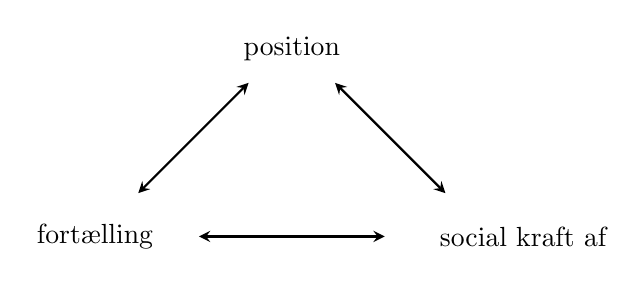
\begin{tikzpicture}[
      scale=0.5,
      trans/.style={thick,<->,shorten >=2pt,shorten 
      <=2pt,>=stealth},
    ]
    \draw[trans] node {fortælling} (1,1) -- (4,4) node[above, 
    xshift=0.5cm, yshift=0.1cm] {position};
    \draw[trans] (6,4) -- (9,1);
    \draw[trans] (2.5,0) -- (7.5,0) node[right, xshift=0.5cm] 
  {social kraft af}; \end{tikzpicture}
  }
}
\caption{De tre gensidigt afhængige elementer i en situation}
\end{figure}
